\section{Materials and methods}
\subsection{Cohort and provenance}
The cohort comprised 278 pelvic models (150 female, 128 male), aged 16--91 years (mean $\pm$ SD: $53.9\pm19.3$ years), using the BoneDat morphology workflow \citep{HenyssKuchar2025BoneDat}. These subjects are a subset of the 281-subject CT collection used in the earlier auricular morphology study \citep{HenysHammer2025}; they are not an independent replication cohort. The present analysis uses the 278 subjects represented in the matched geometry--density simulation archives. Demographic, morphometric and size tables were joined by subject identifier. Eight morphometric variables and the kinematic outcomes were complete for the included cohort (Table~\ref{tab:cohort}). Ethical approval was granted by University Hospital Hradec Kr\'alov\'e, reference 202411IO3P, with waiver of informed consent.
\begin{table}[htbp]
\centering
\caption{Demographic and morphometric characteristics. Values are mean $\pm$ SD; linear dimensions and the subpubic angle are measured from mapped landmarks. Bony pelvic volume sums the selected left and right hip-bone bodies and sacrum.}
\label{tab:cohort}
\StdTableInput{tables/generated/table1_cohort.tex}
\end{table}

\subsection{Anatomical dimensions and their landmarks}
Figure~\ref{fig:morphometry} shows all eight morphometric measures in Table~\ref{tab:cohort}, using the template landmarks from the measurement workflow. Each of the seven linear dimensions is the three-dimensional Euclidean distance $d=\|\mathbf p_2-\mathbf p_1\|$, rather than its projection into a display plane. The subpubic angle uses the second of three landmarks as its vertex:
\begin{equation}
\alpha_{sub}=\arccos\!\left[\frac{(\mathbf p_1-\mathbf p_2)\cdot(\mathbf p_3-\mathbf p_2)}{\|\mathbf p_1-\mathbf p_2\|\,\|\mathbf p_3-\mathbf p_2\|}\right],
\end{equation}
with numerical clipping to $[-1,1]$ and conversion to degrees. The landmark labels are local to each measurement. Landmarks were mapped from the template to each subject; interpolation settings and numerical checks are given in Appendix~\ref{app:implementation_checks}. Total mapped bony pelvic volume is the summed geometric volume of the selected left and right hip-bone bodies (LI and RI in the implementation) and sacrum, expressed in cm$^3$. It excludes the lumbar vertebrae and pelvic canal space and is not a direct measure of cortical-tissue volume. Supplementary Figure S2 illustrates these three bone bodies, the rotational coordinates and point-translation definition.

\begin{figure}[p]
\centering
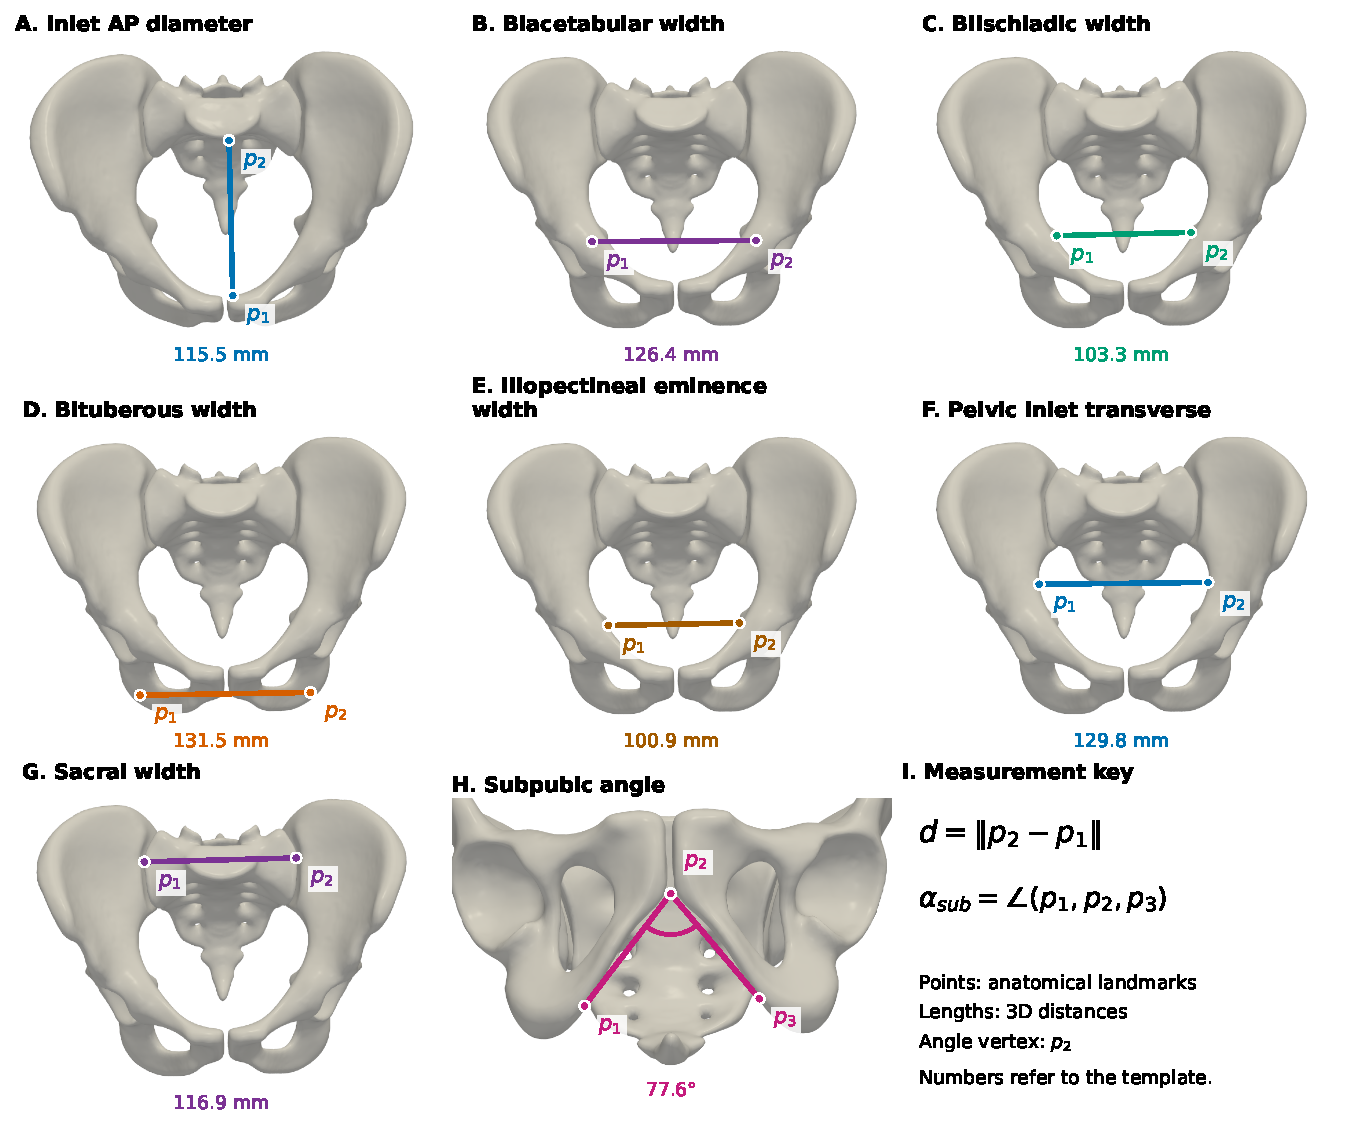
\includegraphics[width=\textwidth,height=0.76\textheight,keepaspectratio]{figures/Fig_morphometric_landmarks.pdf}
\caption{\textbf{Anatomical landmarks for all morphometric measures.} (A--G) Landmark pairs define the seven linear dimensions in Table~\ref{tab:cohort}. (H) The subpubic angle has vertex $p_2$ and arms toward $p_1$ and $p_3$; the view is normal to their plane. (I) Measurement definitions and landmark key. Markers and segments are overlaid on the reference pelvic geometry to keep internal landmarks visible. Values describe the template, not cohort averages. Lengths are measured in three dimensions; each camera direction is perpendicular to its measurement segment. Panels use different views and magnifications.}
\label{fig:morphometry}
\end{figure}

\subsection{Finite-element model}
The simulations used DOLFINx 0.10 on a mesh with 166,808 cells and 48,291 nodes. Small-strain linear elasticity was discretized with four-node tetrahedra and continuous, first-order Lagrange displacement and geometry fields; material properties were cellwise constant (DG0). PETSc used a direct MUMPS LU factorization on the shared reference domain (Appendix~\ref{app:implementation_checks}). Subject anatomy was established by bijective anatomical registration and represented on the FE discretization by $\mathbf{x}=\mathbf{X}+\boldsymbol{\phi}_i(\mathbf{X})$, using radial basis function (RBF) interpolation of the established registration displacement map. Spatial gradients and integration measures were pulled back to the reference domain \citep{BonetWood2008}. This interpolation approximates individual anatomy on a shared discretization and does not reproduce cortical boundaries exactly.

Experimental relationships between bone density and stiffness motivate density-dependent material assignment \citep{Keller1994}. Bone stiffness was assigned using the following bone-modulus approximation:
\begin{equation}
E/\mathrm{MPa}=\begin{cases}
2398, & \rho_{\mathrm{ash}}\le0.486,\\
10200\rho_{\mathrm{ash}}^2, & \rho_{\mathrm{ash}}>0.486,
\end{cases}
\qquad \rho_{\mathrm{ash}}=(\rho+0.09)/1.14,
\end{equation}
where numerical density values are in g\,cm$^{-3}$ and $\rho$ denotes the mapped hydroxyapatite-density input. The implemented approximation comprises this equation, density conversion and low-density floor. The constant low-density branch suppresses modulus variation below its threshold. Bone Poisson ratio was 0.30. Both SIJ cartilage and pubic symphysis used $E=1.0$~MPa and $\nu=0.45$ in all three model variants. These nominal choices were not calibrated to individual subjects.

Ligaments were assembled as linear spring stiffness matrices with a geometric stiffness contribution from prescribed pretension and a pretension force vector. The implementation does not update a tension-only active set during the static solve. Bilateral anterior SIJ, posterior SIJ, interosseous, sacrospinous and sacrotuberous bundles and the pubic bundle were included. Per-bundle stiffnesses were respectively 1400, 5600, 200, 3000, 3000 and 1000~N/mm; total pretension was 20~N per bundle. Each bundle's parameters were divided among its segments. Bone--cartilage interfaces were conforming; frictional contact and muscle activation were not modeled.

\subsection{Loads and constraints}
The superior S1 endplate was constrained using a surface penalty $\gamma=10^6$~N/mm$^3$ (Appendix~\ref{app:mathematical_formulation}). Figure~\ref{fig:overview} shows the load application sites; Table~\ref{tab:loads} gives force vectors in the simulation's global coordinates; these must be distinguished from the subsequently constructed pelvis-aligned reporting frame. SP2leg applies $+400$~N vertically to each acetabulum, and SP1leg applies $+800$~N to the right acetabulum. LAB1 applies opposing ML forces of $\pm400$~N to the internal ring surfaces; LAB2 applies the same signed pair to the ischial tuberosities; LAB3 applies opposing AP forces of $\pm400$~N at the pubis and sacrococcygeal junction. The reference template places both left application patches at greater global $x$ than their right counterparts; thus both ML pairs point outward in that template, consistent with outward loading at both sites. We name the cases by application site because a force direction does not establish the direction of joint motion.

Surface tractions were normalized by mapped surface area, giving identical prescribed force resultants across subjects. LAB force pairs have zero net force, whereas standing cases have an 800~N net vertical force balanced by the sacral constraint. Equal sums of force magnitudes do not imply equal moments, work, or physiological demand. The analyses compare responses to these standardized mechanical probes. All load cases include the prescribed ligament pretension.
\begin{table}[htbp]
\centering
\caption{Standardized loads in global simulation coordinates. LAB1--LAB3 are independent mechanical proxies.}
\label{tab:loads}
\StdTableInput{tables/generated/table2_loads.tex}
\end{table}

\subsection{Reference configuration and SIJ kinematics}
The kinematic analysis compares each unloaded mapped surface $\mathbf{x}^0_i=\mathbf{X}+\boldsymbol{\phi}_i$ with its loaded surface $\mathbf{x}^1_{i\ell}=\mathbf{x}^0_i+\mathbf{u}_{i\ell}$. The reference is the anatomical configuration with zero elastic displacement; a separately equilibrated pretension-only configuration is not used. Absolute motion therefore describes the combined external-load and prescribed-ligament-pretension solution relative to this anatomical reference. Pretension is a model assumption, not an experimentally measured subject-specific value. Correspondence and pairing checks are documented in Appendix~\ref{app:implementation_checks}.



Relative ilium-to-sacrum motion was estimated using trimmed Kabsch registration of opposing surface regions within 5~mm, with a minimum of 80 nodes per region. The underlying least-squares rigid fit follows \citet{Kabsch1976}; trimming and ROI selection are implementation choices. Before registration, the inverse least-squares affine sacral map was applied to all loaded points. This removes sacral affine strain as well as rigid drift; the resulting quantities are affine-corrected relative motion, rather than unmodified physical joint displacement. The available rigid-only sensitivity check is reported below.

Motion was expressed in a pelvis-aligned ML/AP/CC frame, not a local articular normal/tangent frame. Fixed-axis Cardan $xyz$ angles satisfy $R=R_zR_yR_x$. The bilateral mean of the Euclidean norms of these angle triplets is denoted $|\boldsymbol{\theta}|$; this is a small-angle summary, not the exact invariant rotation angle. Translation $|\mathbf d|$ is the bilateral mean of the norms of relative displacements evaluated at the sacral ROI centroid. Component summaries are bilateral means of absolute values. In particular, $|\theta_x|$ does not distinguish nutation from counternutation, and $|d_{ML}|$ is not a measurement of joint gapping. Translation-magnitude asymmetry is $\big|\|\mathbf d_L\|-\|\mathbf d_R\|\big|$.

\subsection{Matched variants and variance ratios}
The full variant uses subject-specific geometry and bone density. The geometry-preserved / standardized-density variant (G) retains subject geometry, including scale, and uses the spatially varying pointwise population-median density field; it is not homogeneous bone. The density-preserved / template-geometry variant (D) uses subject density on the template geometry. Cartilage and ligament parameters remain nominal in all variants.

For each load and endpoint we calculated $100V_G/V_{full}$ and $100V_D/V_{full}$, with 2000 paired subject bootstrap samples \citep{EfronTibshirani1994}. These non-additive ratios can exceed 100\% and neither estimate causal variance fractions nor separate geometry--material interactions. Geometry-preserved/full agreement was also assessed by RMSE, MAE and identity-line $R^2=1-\sum_i(Y_{G,i}-Y_{full,i})^2/\sum_i(Y_{full,i}-\bar Y_{full})^2$.

\subsection{Prediction from size and a limited anatomical description}
The central predictive comparison used load-specific OLS models for $\log Y$, with $Y$ equal to rotation or translation magnitude. The size model used age and $\log V$. The triad model added inlet AP diameter, interspinous width and subpubic angle. Two benchmark models added, respectively, female sex and its interaction with $\log V$ to the triad, or replaced the triad with all eight available morphometric measures. Sex was not an independent parameter of the FE constitutive model. Predictor sets were fixed for this retrospective comparison; the original selection of the triad was not repeated within validation folds.

We used ten repeats of ten-fold cross-validation, stratified by sex at the subject level (random seed 20261002 plus repeat index). The same folds were used for every outcome, load and predictor set. All observations of a held-out subject were excluded from training; load-specific models were fitted only to the training subjects. Predictors were standardized using each training fold. Predictions on the arithmetic outcome scale used a training-only smearing factor, $\widehat Y=\exp(\widehat{\log Y})\,n_{train}^{-1}\sum_{i\in train}\exp(e_i)$. Each fold fitted the predefined predictor set without further feature selection or hyperparameter tuning.

Reported RMSE and MAE pool all held-out predictions across repeats. Prediction $R^2=1-\operatorname{mean}_{i,r}(Y_i-\widehat Y_{ir})^2/\operatorname{var}_i(Y_i)$ uses the cohort outcome variance, separately for each load and endpoint; it is not training fit. Paired gains compare models on identical held-out observations. Pointwise 95\% bootstrap intervals use 3000 subject resamples of repeat-averaged squared errors, preserving pairing across predictor sets. They condition on fitted cross-validation predictions and do not include the uncertainty of refitting or retrospectively selecting the triad. Repeated folds are not treated as independent samples. Validation addresses new subjects from the represented population under each specified load, not external specimens or unseen loading configurations.

\subsection{Controlled test of a directional limit to scalar prediction}
We redistributed each 400~N transverse side force between the internal-ring (LAB1) and ischial (LAB2) patches. At fraction $w\in\{0,0.25,0.5,0.75,1\}$, LAB1 patches receive fraction $1-w$ and LAB2 patches fraction $w$. Each side's total force and direction remain unchanged; geometry, density, constraints and linearized tissue stiffness remain fixed. Because both endpoint solutions contain the same pretension and the weights sum to one, the displacement field
\begin{equation}
\mathbf u_i(w)=(1-w)\mathbf u_{i,LAB1}+w\mathbf u_{i,LAB2}
\label{eq:mixture_field}
\end{equation}
solves the corresponding mixed-force problem in the implemented linear system. The experiment uses exact field superposition and requires no new FE factorization.

For all 278 subjects, motion was re-extracted from the mixed fields using the original affine-corrected, trimmed-Kabsch definitions and each subject's fixed unloaded ROI. Both endpoint weights reproduced the archived corrected rotations and translations to absolute and relative tolerances of $10^{-8}$. A scalar endpoint estimate combines bilateral translation magnitudes, $S_i(w)=(1-w)Y_{i,LAB1}+wY_{i,LAB2}$. A signed-vector endpoint estimate first combines each side's reported displacement vectors and then takes their bilateral mean norm, $D_i(w)=\frac12\sum_{s=L,R}\|(1-w)\mathbf d_{i,LAB1,s}+w\mathbf d_{i,LAB2,s}\|$.

The vector norm contains the cross-term $2w(1-w)\mathbf d_{LAB1,s}\cdot\mathbf d_{LAB2,s}$, which scalar magnitudes cannot identify. We quantified the reduction relative to scalar combination as $100[1-Y_i(w)/S_i(w)]$ and compared scalar and vector RMSE against re-extracted $Y_i(w)$. Signed-vector combination is an approximation at the level of these fitted kinematic outputs, despite exact superposition of the underlying FE fields; its error was measured rather than assumed zero. Both endpoint estimates use individual FE endpoint information and are mechanism diagnostics, not anatomy-only held-out predictions. This experiment tests transfer to a controlled load mixture; it does not identify the causes of residual cross-subject prediction error. Bootstrap intervals for median reduction use 3000 subject resamples.

\subsection{Statistical analysis}
All comparisons were retrospective and were not preregistered. Held-out prediction gains and the controlled load-mixture experiment form the central analyses; anatomical-adjustment, load-profile and density-variant comparisons provide context and delimit their interpretation. Distributions are summarized by medians and interquartile ranges. Paired component contrasts use $\Delta_{i\ell,k}=|d_k|_{i\ell}-|d_k|_{i,SP2leg}$, with 3000 subject bootstrap samples for median confidence intervals and two-sided exact binomial sign tests (zero differences excluded). Wilcoxon signed-rank statistics \citep{Wilcoxon1945} are retained in the machine-readable output as a sensitivity diagnostic, but are not used for primary inference because asymmetric differences can yield a signed-rank result that disagrees with the direction of the median. Benjamini--Hochberg correction was applied to the 12 component comparisons \citep{BenjaminiHochberg1995}. Bilateral versus unilateral support uses a separate three-test family for rotation magnitude, translation magnitude and translation asymmetry. Direct LAB2-minus-LAB1 contrasts use a separate three-component family. Prediction-gain intervals are descriptive, pointwise comparisons of paired held-out errors; no multiplicity-adjusted hypothesis tests were applied to them.

For each LAB case, nested OLS models used HC3 covariance \citep{MacKinnonWhite1985}:
\begin{align}
\mathrm{M0}:\quad Y&=\beta_0+\beta_s\mathrm{Female}+\beta_a\mathrm{Age}_z+\epsilon,\label{eq:m0}\\
\mathrm{M1}:\quad Y&=\mathrm{M0}+\beta_v\log(V)_z,\label{eq:m1}\\
\mathrm{M2}:\quad Y&=\mathrm{M1}+\beta_{AP}\mathrm{AP}_z+\beta_b\mathrm{Biischiadic}_z+\beta_p\mathrm{Subpubic}_z.\label{eq:m2}
\end{align}
Here model addition denotes addition to the linear predictor. Female is coded 1 and male 0; continuous predictors are standardized using cohort sample SDs. M2 contains no sex--volume interaction. FDR correction covers its six sex coefficients (two outcomes by three loads). M0/M1 and coefficient attenuation are descriptive. VIFs quantify collinearity without treating a threshold as proof of identifiability. The triad describes inlet depth, interspinous midpelvic width and the anterior pubic arch; it was selected for this retrospective analysis. Pooled and sex-stratified Spearman correlations are exploratory, not evidence of mediation.

Pooled OLS models include load, sex, age, log volume, the morphometric triad, load--volume interactions and a sex--volume interaction, with covariance clustered by the 278 subjects \citep{CameronMiller2015}. A main volume coefficient therefore refers to male SP2leg, not an overall pooled slope. FDR is applied within each outcome's pooled coefficients. Robust Wald statistics are not converted to partial variance-explained measures.

Exploratory load-specific association models regress $\log Y$ on $\log V$, sex, their interaction, age and the triad. Male and female slopes are $\beta_v$ and $\beta_v+\beta_{v:s}$; HC3 covariance supplies 95\% Wald intervals. FDR covers 20 sex-specific slope tests, with a separate family of ten interaction tests. Failure to reject an interaction is not evidence of equal slopes. A matched specification omitting the triad assesses the dependence of volume coefficients on anatomical adjustment (Supporting Information, Table S13). Neither specification represents uniform geometric scaling. The alternative $\log(\mathrm{scale})$ model is an algebraic reparameterization because $\log V=3\log(\mathrm{scale})+\log V_{template}$; it is not an independent robustness test. A sensitivity analysis added a quadratic age term to the nested sex models and the conditional volume models (Supporting Information, Tables S7--S8). Sample confidence intervals do not include uncertainty in loads, constitutive choices, segmentation or boundary conditions.
